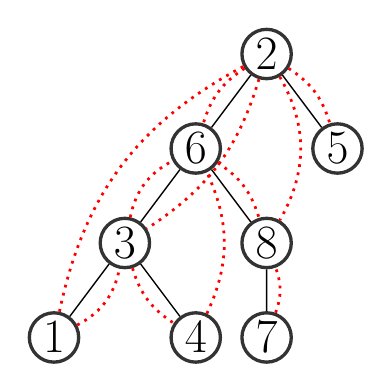
\begin{tikzpicture}[
  grow=down, level distance=12mm, sibling distance=18mm,
  every node/.style={circle, draw=black!80, very thick, inner sep=1.5pt, font=\LARGE, fill=white, text=black},
  edge from parent/.style={draw, line width=0.5pt}
]
  \node (t2) {2} child {node (t6) {6} child {node (t3) {3} child {node (t1) {1}} child {node (t4) {4}}} child {node (t8) {8} child {node (t7) {7}}}} child {node (t5) {5}};
  % original graph edges (dotted, now red and curvy)
  \draw[dotted, red, line width=1pt, bend left=25] (t1) to (t2);
  \draw[dotted, red, line width=1pt, bend right=25] (t1) to (t3);
  \draw[dotted, red, line width=1pt, bend left=20] (t2) to (t3);
  \draw[dotted, red, line width=1pt, bend left=20] (t2) to (t5);
  \draw[dotted, red, line width=1pt, bend right=20] (t2) to (t6);
  \draw[dotted, red, line width=1pt, bend left=30] (t2) to (t8);
  \draw[dotted, red, line width=1pt, bend right=20] (t3) to (t4);
  \draw[dotted, red, line width=1pt, bend left=25] (t3) to (t6);
  \draw[dotted, red, line width=1pt, bend right=25] (t4) to (t6);
  \draw[dotted, red, line width=1pt, bend left=20] (t6) to (t8);
  \draw[dotted, red, line width=1pt, bend right=20] (t7) to (t8);
\end{tikzpicture}
